\documentclass[10pt,aspectratio=169,dvipsnames]{beamer} % sets document type, default font size, slide aspect ratio, and loads color names
\usetheme[color/block=transparent]{metropolis} % sets the theme of the document

\usepackage[absolute,overlay]{textpos} % allows absolute positioning of text
\usepackage{booktabs} % enhances quality of tables
\usepackage[utf8]{inputenc} % allows input encoding in UTF-8
\usepackage{tikz} % used for creating vector graphics
\usetikzlibrary{arrows.meta} % loads additional arrow types
\usepackage[europeanresistors,americaninductors]{circuitikz} % for drawing electrical circuits
\usepackage[scale=2]{ccicons} % loads Creative Commons icons
\usepackage[official]{eurosym} % loads the official symbol for the Euro
\usepackage{hyperref} % allows creating hyperlinks in the document

\newcommand{\ra}[1]{\renewcommand{\arraystretch}{#1}} % creates command to adjust spacing between rows
\newcommand{\hrefc}[2]{\href{#1}{\bf\color{blue}{\underline{#2}}}} % defines command for underlined, blue hyperlink
\newcommand{\urlc}[1]{\hrefc{#1}{#1}} % defines command for URL hyperlink

\newcommand{\R}{\mathbb{R}} % creates a shortcut for typing real numbers symbol
\newcommand{\ubar}[1]{\text{\b{$#1$}}} % defines a command for underlined text

\xdefinecolor{TUred}{RGB}{197,14,31} % defines a new color TUred
\setbeamerfont{alerted text}{series=\bfseries} % sets the font of alerted text to bold
\setbeamercolor{alerted text}{fg=TUred} % sets the color of alerted text to TUred
\setbeamercolor{background canvas}{bg=white} % sets the background color to white
\setbeamercolor{frametitle}{bg=lightgray!40, fg=TUred} % sets the background color of the frame title to light gray and text color to TUred
\setbeamercolor{title}{fg=TUred} % sets the color of the title to TUred

\addtobeamertemplate{frametitle}{}{% adds image to every frame title
  \begin{textblock*}{100mm}(1.01\textwidth,2pt)
    
\includegraphics[width=1.5cm]{images/TUB.png}
    \end{textblock*}}

\def\l{\lambda} % defines a shortcut for lambda symbol
\def\m{\mu} % defines a shortcut for mu symbol
\def\d{\partial} % defines a shortcut for partial symbol
\def\cL{\mathcal{L}} % defines a shortcut for caligraphic L symbol
\def\co{CO${}_2$} % defines a shortcut for CO2 symbol
\def\el{${}_{el}$} % defines a subscript for el
\def\th{${}_{th}$} % defines a subscript for th
\def\gas{${}_{gas}$} % defines a subscript for gas

\setbeamercolor{framesource}{fg=gray} % sets color of framesource to gray
\setbeamerfont{framesource}{size=\tiny} % sets font size of framesource to tiny
\newcommand{\source}[1]{% creates command for inserting a source footnote
\begin{textblock*}{5cm}(10.5cm,8.35cm)
    \begin{beamercolorbox}[ht=0.5cm,right]{framesource}
        \usebeamerfont{framesource}\usebeamercolor[fg]{framesource} {#1}
    \end{beamercolorbox}
\end{textblock*}}

\graphicspath{{../results/}} % sets the path where graphics can be found
\DeclareGraphicsExtensions{.pdf,.jpeg,.png,.jpg} % defines the types of graphic files that can be used

\def\goat#1{{\scriptsize\color{green}{[#1]}}} % defines a command for green, scriptsize text

\let\olditem\item % saves the old item command
\renewcommand{\item}{\olditem\vspace{5pt}} % redefines the item command to add space after each item


\title{System-level impacts of 24/7 carbon-free electricity procurement in Europe}

%\subtitle{---}
\author{
  Iegor Riepin, Tom Brown\\
  \hrefc{https://tub-ensys.github.io/}{Department of Digital Transformation in Energy Systems}, TU Berlin
}

\date{30 September 2022}

\titlegraphic{%
  \vspace{0cm}
  \hspace{10.7cm}
    
\includegraphics[trim=0 0cm 0 0cm,height=1.2cm,clip=true]{images/TUB.png}

\vspace{5.1cm}
   
}


\begin{document}

\maketitle



\begin{frame}
  \frametitle{Acknowledgements}

  \begin{itemize}
    \item {\bf Funding:} This study was supported by a grant from Google, Inc. 
    \item {\bf Acknowledgements:} The authors acknowledge members of the Google energy markets and policy team 
    for their feedback and inputs on earlier drafts of this report. 
    Also, warm regards to the \hrefc{https://pypsa.org/}{PyPSA team} and many contributors to the open-source 
    PyPSA energy system modelling tool used in this study (see: \hrefc{https://github.com/PyPSA/PyPSA}{github.com/PyPSA})
    \item 
    {\bf Copyright} Unless otherwise stated, graphics and text are Copyright \copyright Tom Brown and Iegor Riepin, 2022.
    Graphics and text for which no other attribution are given are licensed under a 
    \href{https://creativecommons.org/licenses/by/4.0/}{CC BY 4.0}.  {\footnotesize \ccby} 
    \item The content of this study, including any errors or omissions are the responsibility
    of the authors alone.
  \end{itemize}

\end{frame}


\begin{frame}

  \frametitle{Table of Contents}
  \setbeamertemplate{section in toc}[sections numbered]
  \tableofcontents[hideallsubsections]
\end{frame}


%----------------------------------------
%----------------------------------------

\section{Introduction}


\begin{frame}{Introduction}

  \centering
    \begin{itemize}
    \item Climate change is driving a global effort to rapidly decarbonise 
    electricity systems across the globe. 
    Many public and private energy buyers have joined this effort and highlight
    their sustainable credentials by procuring renewable energy with the 
    Power Purchase Agreements (PPAs).
    \item Such \alert{voluntary commitments accelerate the deployment of renewable 
    capacity} above the policy requirements in the countries and jurisdictions
    these companies operate. This facilitates faster
    transformation of electricity markets by driving renewables
    techologies down the experience curves.
    \item Additionally, many early actors in the field helped pave the way for followers 
    \hrefc{https://www.gstatic.com/gumdrop/sustainability/247-carbon-free-energy.pdf}{by 
    developing methods and establishing standard contracts} for clean energy procurement.
    \end{itemize}
  
\end{frame}


\begin{frame}{Introduction}

  \begin{columns}[T]
    \begin{column}{6cm}
      \begin{itemize}
        \item   PPAs typically allow for renewable energy to match supply and
        demand on average over a long period of time. 
        \item For example, more than 370 members of the \href{https://www.there100.org/}{RE100} group have committed to purchasing enough renewable energy to match
        \alert{100\% of their electricity consumption on an annual basis}.
      \end{itemize}
    \end{column}

  \begin{column}{10cm}
      \centering
      
      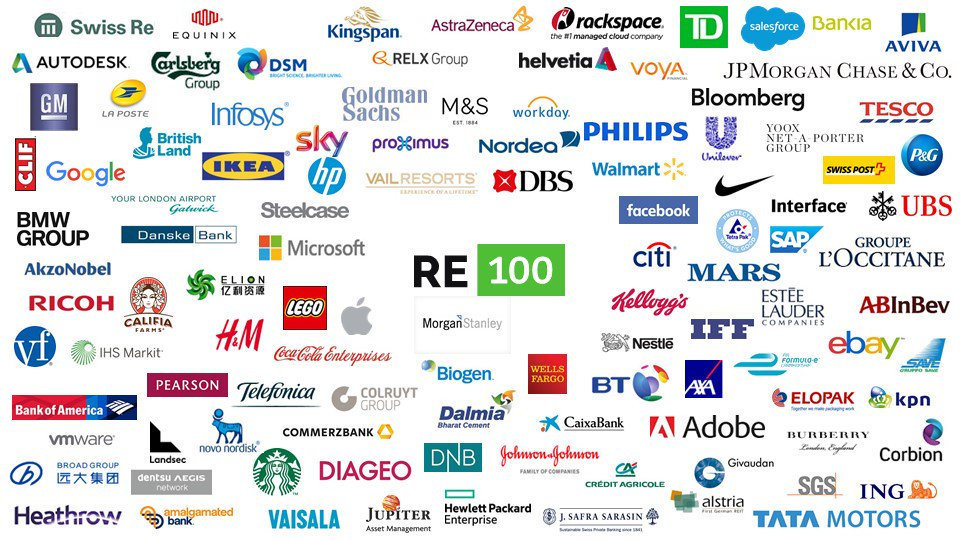
\includegraphics[width=10cm]{images/100re-companies.jpg}
      \vspace{.1cm}
      More than 370 companies have joined \hrefc{https://www.there100.org/}{RE100}
    \end{column}
    \end{columns}

    \source{source: \href{https://www.there100.org/}{RE100}}
\end{frame}
  

\begin{frame}{Introduction}
  
    \begin{itemize}
    \item However, electricity buyers that commit to 100\% annual matching 
    from renewable energy sources still face times when generation 
    from wind and solar generators is not sufficient to match 
    the companies’ electricity demand. 
    \item Thus, although buyers match their demand on a \alert{yearly} basis with 
    renewable energy, on an \alert{hourly} basis they still have hours 
    when they have to rely on carbon-emitting technologies available 
    on a local market, such as coal and gas-fired power plants.
    \end{itemize}

  \centering
  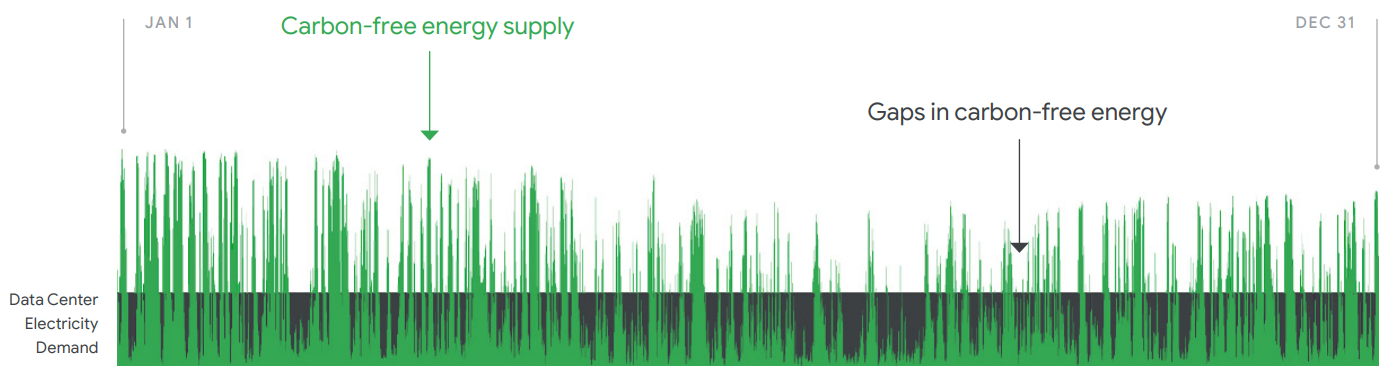
\includegraphics[width=14cm]{images/google-year.png}
  \source{\href{https://www.gstatic.com/gumdrop/sustainability/247-carbon-free-energy.pdf}{source: Google 24/7 CFE}}
           
\end{frame}


\begin{frame}{Introduction}
  
  More generally, 100\% annual matching leads to many challenges 
  from the electricity buyers' and system perspectives: 
  \begin{itemize}
  \item No \alert{simultaneity} - variable generation of wind and solar power is not aligned with the 
  buyer’s electricity consumption profile.
  \item Lack of \alert{additionality} - some buyers procure unbundled guarantees of origin from existing 
  facilities, which does not lead to additional renewable generation.
  \item Displaced \alert{location} - some buyers procure  PPAs from locations far away from their consumption.
  \item Exposure to \alert{risk} - electricity buyers are exposed to price volatility 
  in local electricity markets.
  \item Need for \alert{backup} - electricity system has to maintain backup and flexibility options 
  for hours with low renewable generation.
  \end{itemize}
  
\end{frame}


\begin{frame}{Introduction}

  \centering

  There is growing interest from leaders in voluntary clean
  electricity procurement to cover their consumption 
  with clean energy supply on a \alert{truly 24/7 basis}. \\
  \vspace{0.3cm}
  Achieving 24/7 Carbon-Free Energy (CFE) means that every kilowatt-hour of electricity consumption is met
  with carbon-free electricity sources, \alert{every hour of every day}.
  
\end{frame}


\begin{frame}{Introduction}
  
  \begin{columns}[T]
  \begin{column}{8cm}

    \begin{itemize}
    \item The \hrefc{https://www.un.org/en/energy-compacts/page/compact-247-carbon-free-energy}{24/7 Carbon-free Energy Compact} 
    initiative was launched in 2021 by Sustainable Energy for All and the United Nations. 
    It now includes more than 80 companies, policymakers, investors, and organizations 
    on a mission to realize a 24/7 Carbon-Free Energy future. 

    \item One of the forefront runners in 24/7 initiative is Google Inc. In 2020 the company committed 
    \hrefc{https://www.gstatic.com/gumdrop/sustainability/247-carbon-free-energy.pdf}{to the goal} 
    of operating entirely on a 24/7-CFE approach at all its data centres and campuses worldwide by 2030. 
    Shortly after, Google published 
    \hrefc{https://www.gstatic.com/gumdrop/sustainability/policy-roadmap-carbon-free-energy.pdf}{a policy roadmap} 
    on achieving the 24/7-CFE goal.

    \end{itemize}
  \end{column}

  \begin{column}{8cm}
    \centering
    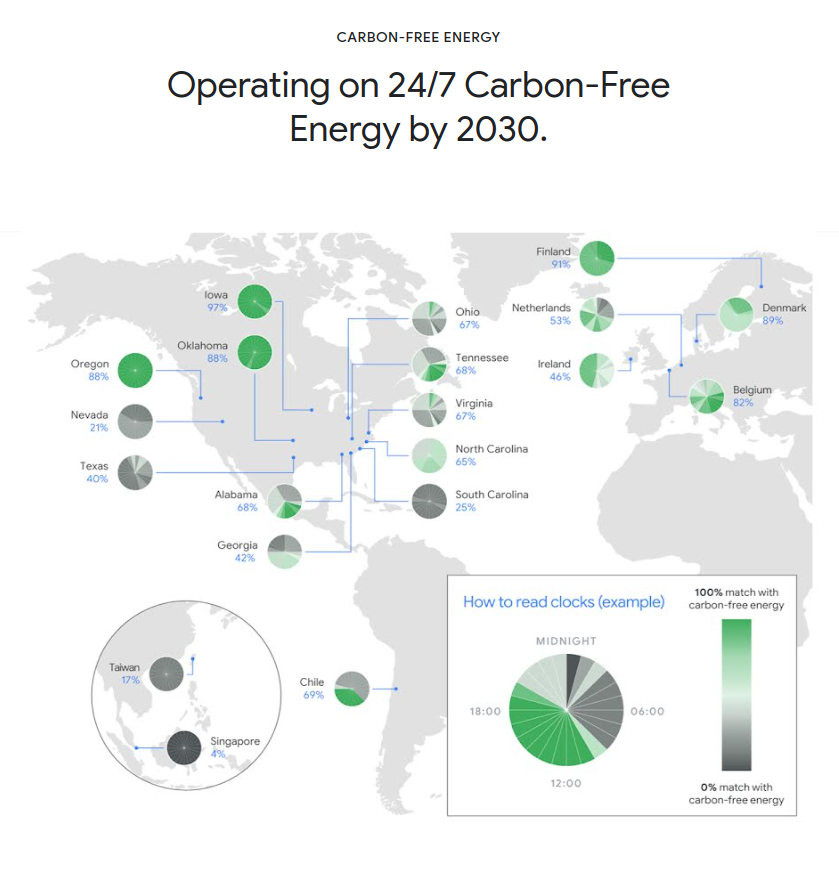
\includegraphics[width=7.5cm]{images/247-google-web.png}
    \vspace{.1cm}
  \end{column}

  \source{\href{https://sustainability.google/progress/energy/}{Google Inc.}}
  \end{columns}
  
\end{frame}


\begin{frame}{Introduction}
  
  The 24/7 CFE procurement has potential benefits over the 100\% renewable matching:
  
  \begin{itemize}
  \item Ensure match of electricity consumption with carbon-free resources 
        on an \alert{hourly basis}.
  \item Enable much \alert{deeper reductions in CO$_2$} emissions assosiated 
        to buyer's electricity consumption.
  \item Ensure that contracted power is \alert{additional} (i.e. leads to new capacity).
  \item Ensure that power comes from the \alert{same bidding zone}.
  \item Enable procurement of \alert{carbon-free} rather than renewable technologies 
        (such as advanced “clean dispatchable” power generation and long-duration energy storage).
  \end{itemize}
  
\end{frame}


\begin{frame}{Focus of the study}
  
  In this study, we investigate both the \alert{means and costs of 24/7 procurement} for companies
  and the \alert{system impacts} for the rest of the European electricity system. 

  We focus our analysis on the following quesitons:

    \begin{enumerate}
    \item How can companies following 24/7~CFE procurement achieve hourly matching?
    \item What is the cost premium of 24/7~CFE versus the 100\% annual matching?
    \item To which extent can technologies, such as long-duration storage or advanced dispatchable
          clean generators, help to achieve the 24/7~CFE goal?
    \item To which extent can 24/7~CFE contribute to reductions in CO$_2$
          emissions intensity of buyer's consumption? 
    \item If many companies follow the 24/7~CFE approach, how does this effect the rest of
          the energy system?
    \end{enumerate}
  
\end{frame}



\begin{frame}{Quick summary}
  
  \begin{columns}[T]
  \begin{column}{9cm}
  \centering

    \begin{itemize}
    \item Key findings
    \end{itemize}
  \end{column}
  \end{columns}
  
\end{frame}

%----------------------------------------
%----------------------------------------

\section{Summary of study design}

\begin{frame}
  \frametitle{Open Model of European Energy System: PyPSA-Eur(-Sec)}

\begin{columns}[T]
\begin{column}{6cm}

  \begin{itemize}

  \item PyPSA is an \alert{open source} tool for modelling energy systems developed at TU Berlin
  \item PyPSA is used worldwide by \alert{dozens of research institutes and companies}. See \hrefc{https://pypsa.readthedocs.io/en/latest/users.html}{list of users}
  \item PyPSA-Eur is an open model of the European power system at the transmission network level that covers the \alert{full ENTSO-E area}
  \end{itemize}

\end{column}

\begin{column}{8cm}

\centering
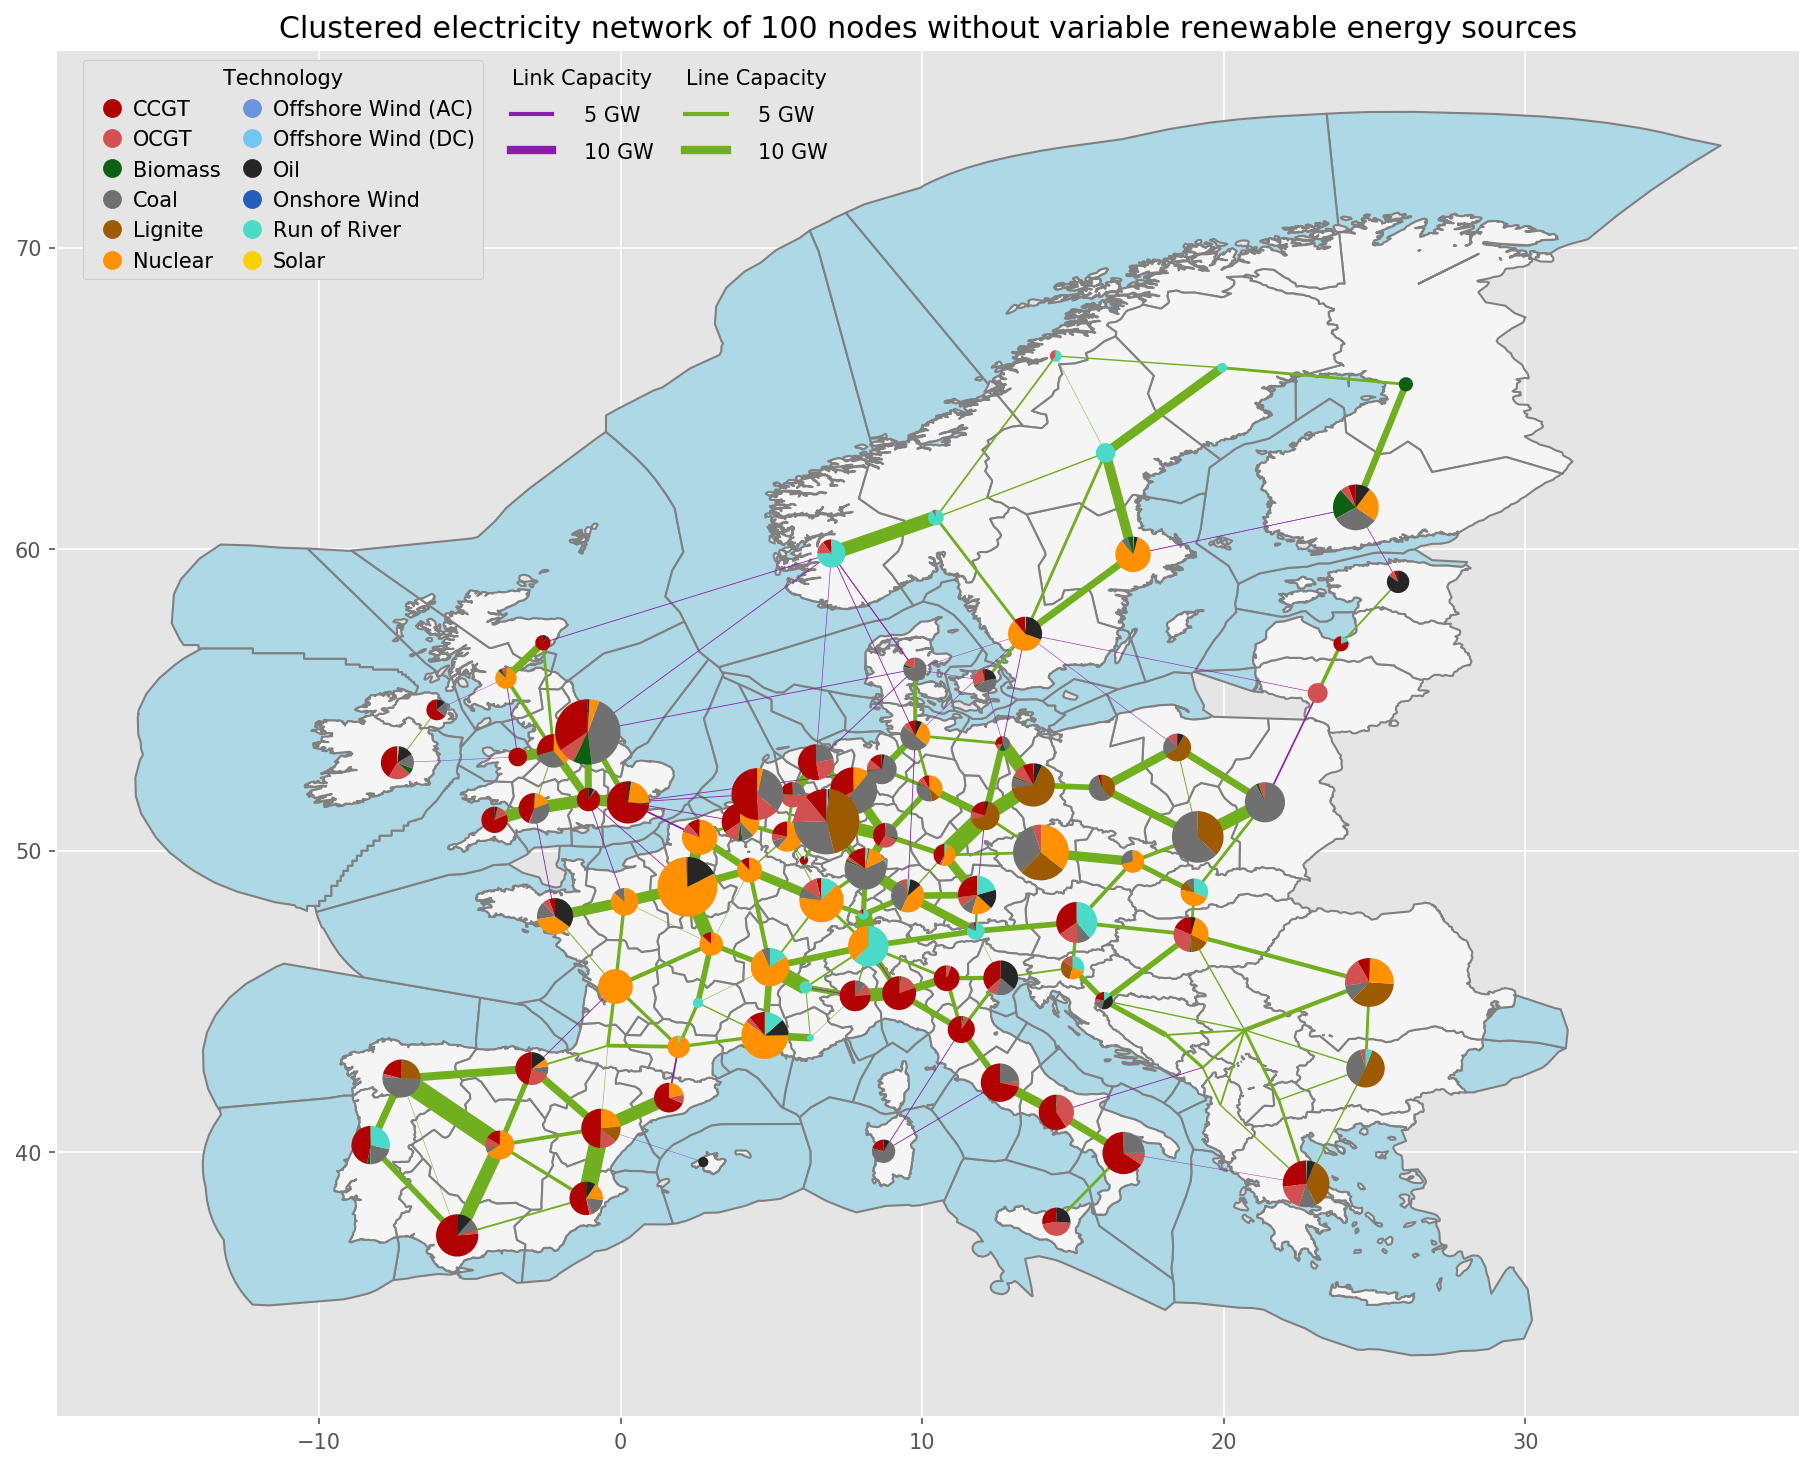
\includegraphics[width=8cm]{images/elec_s_100.png}

 \vspace{0.1cm}

 PyPSA-Eur(-Sec) suite of models are available on \hrefc{https://pypsa.org/}{GitHub}

\end{column}
\end{columns}

\end{frame}

%----------------------------------------

\begin{frame}
  \frametitle{Study design 1/2}

\begin{columns}[T]
\begin{column}{6cm}

  \begin{itemize}

  \item We model the European power system consisting of \alert{37 zones}
  \item C\&I taking 24/7 approach can be located in either of the \alert{four zones}: Ireland, Denmark (zone DK1 or DK-West), Germany and the Netherlands
  \item Different shares of national C\&I demand participate in 24/7 approach. We assume here \alert{10\%} and \alert{25\%}
  \end{itemize}

\end{column}

\begin{column}{8cm}

\centering
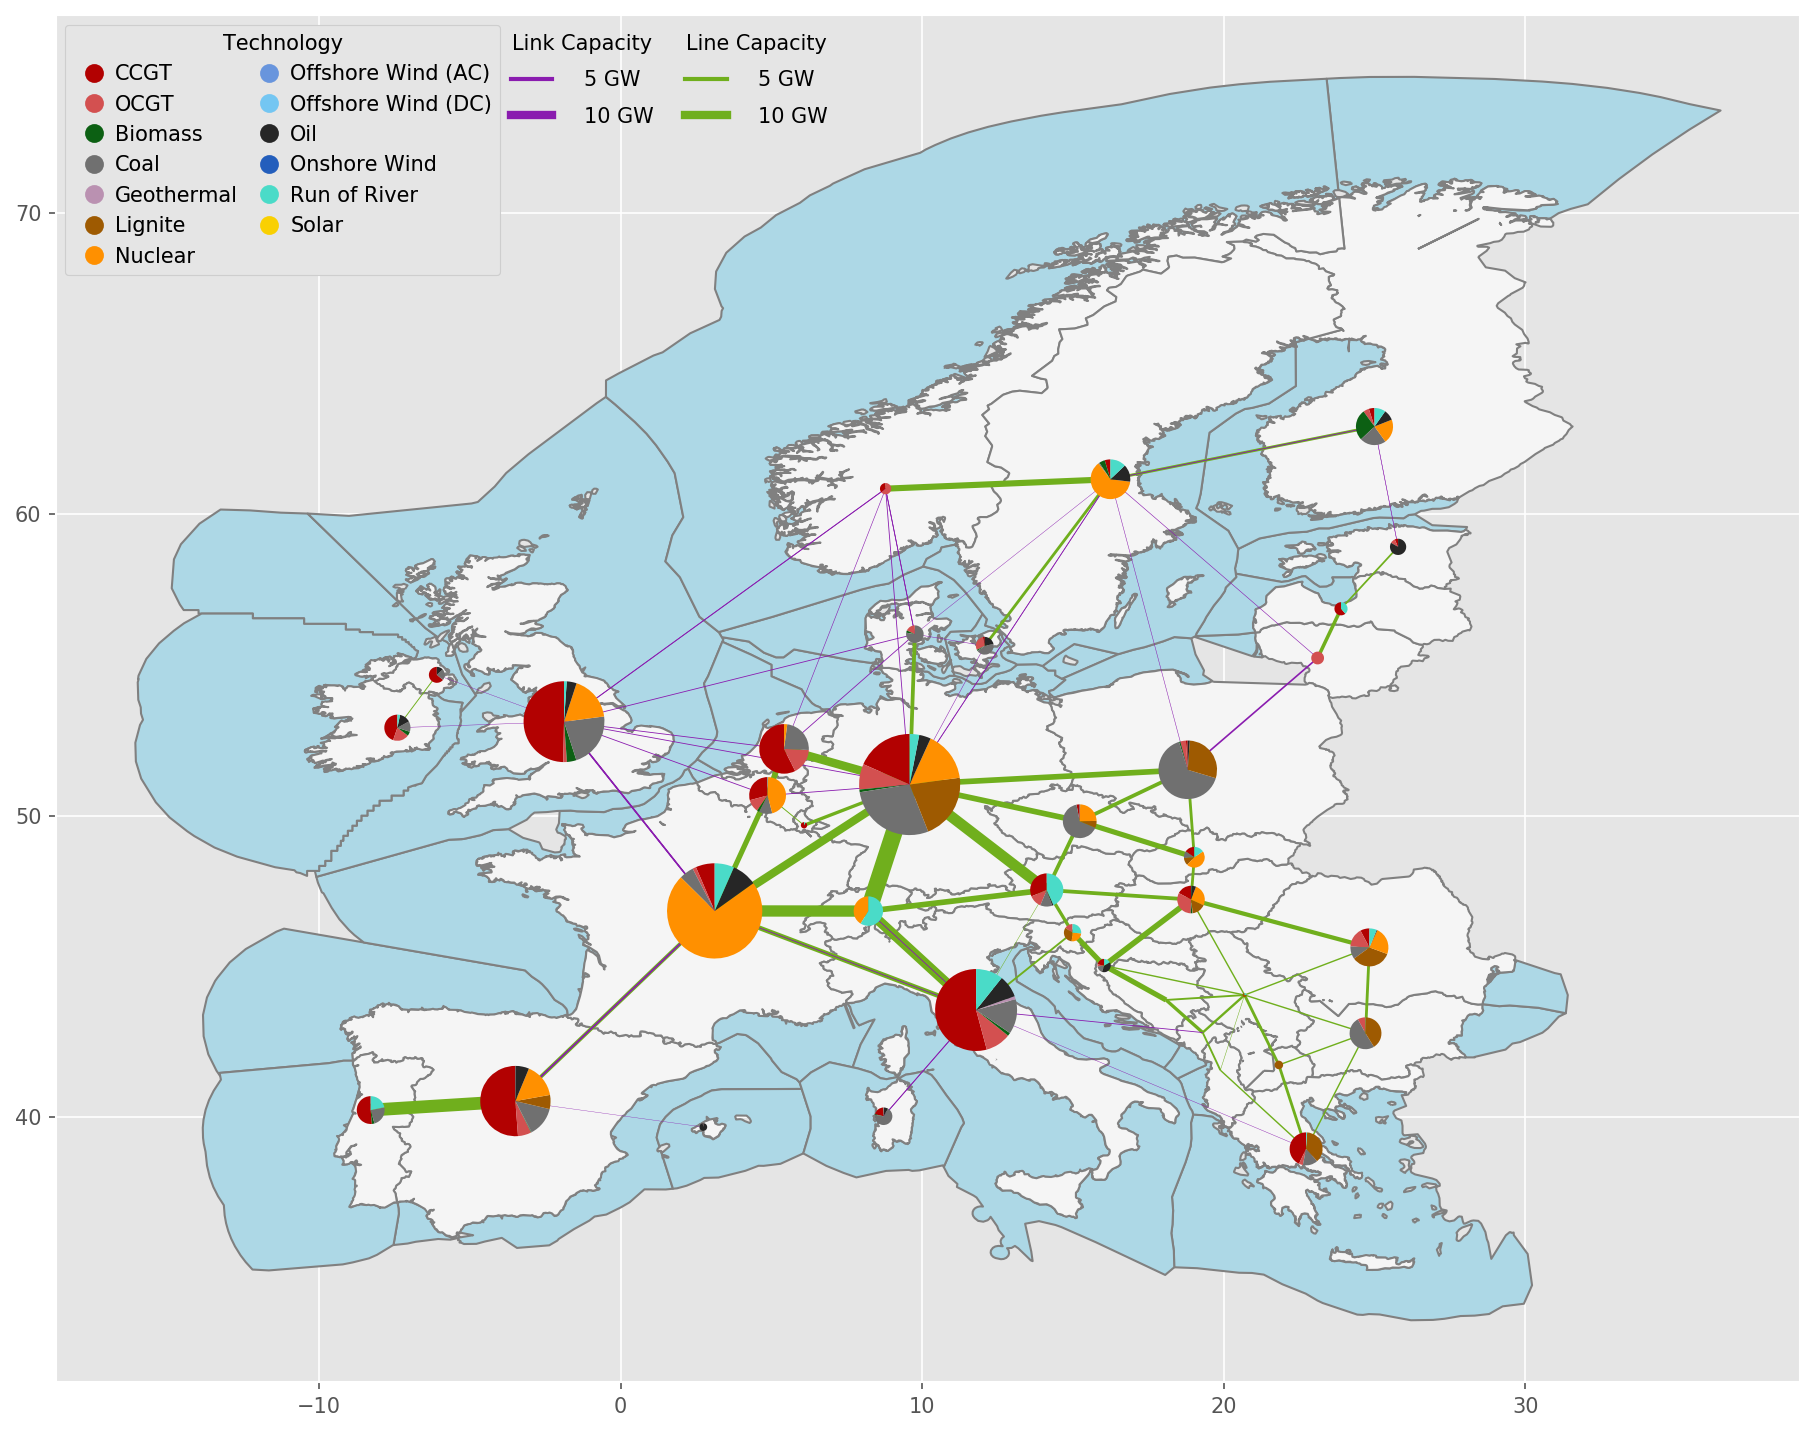
\includegraphics[width=8cm]{images/elec_s_37.png}

\vspace{0.1cm}
PyPSA-Eur network clustered to 37 zones

\end{column}
\end{columns}

\end{frame}

%----------------------------------------

\begin{frame}
  \frametitle{Study design 2/2}

\begin{columns}[T]
\begin{column}{6cm}

  \begin{itemize}

  \item We focus on two periods: \\ \alert{2025} and \alert{2030}. Periods differ by \\ 
  (i) technology cost assumptions, \\ 
  (ii) renewable expansion pathways (based on NECPs), \\(iii) \emph{brownfield} fleet of power plants
  \item We incorporate various technologies that can be procured by C\&I customers: wind, solar, short-term storage (batteries), long-term storage (hydrogen storage system), and advanced geothermal system
  \end{itemize}

\end{column}

\begin{column}{8cm}

\centering
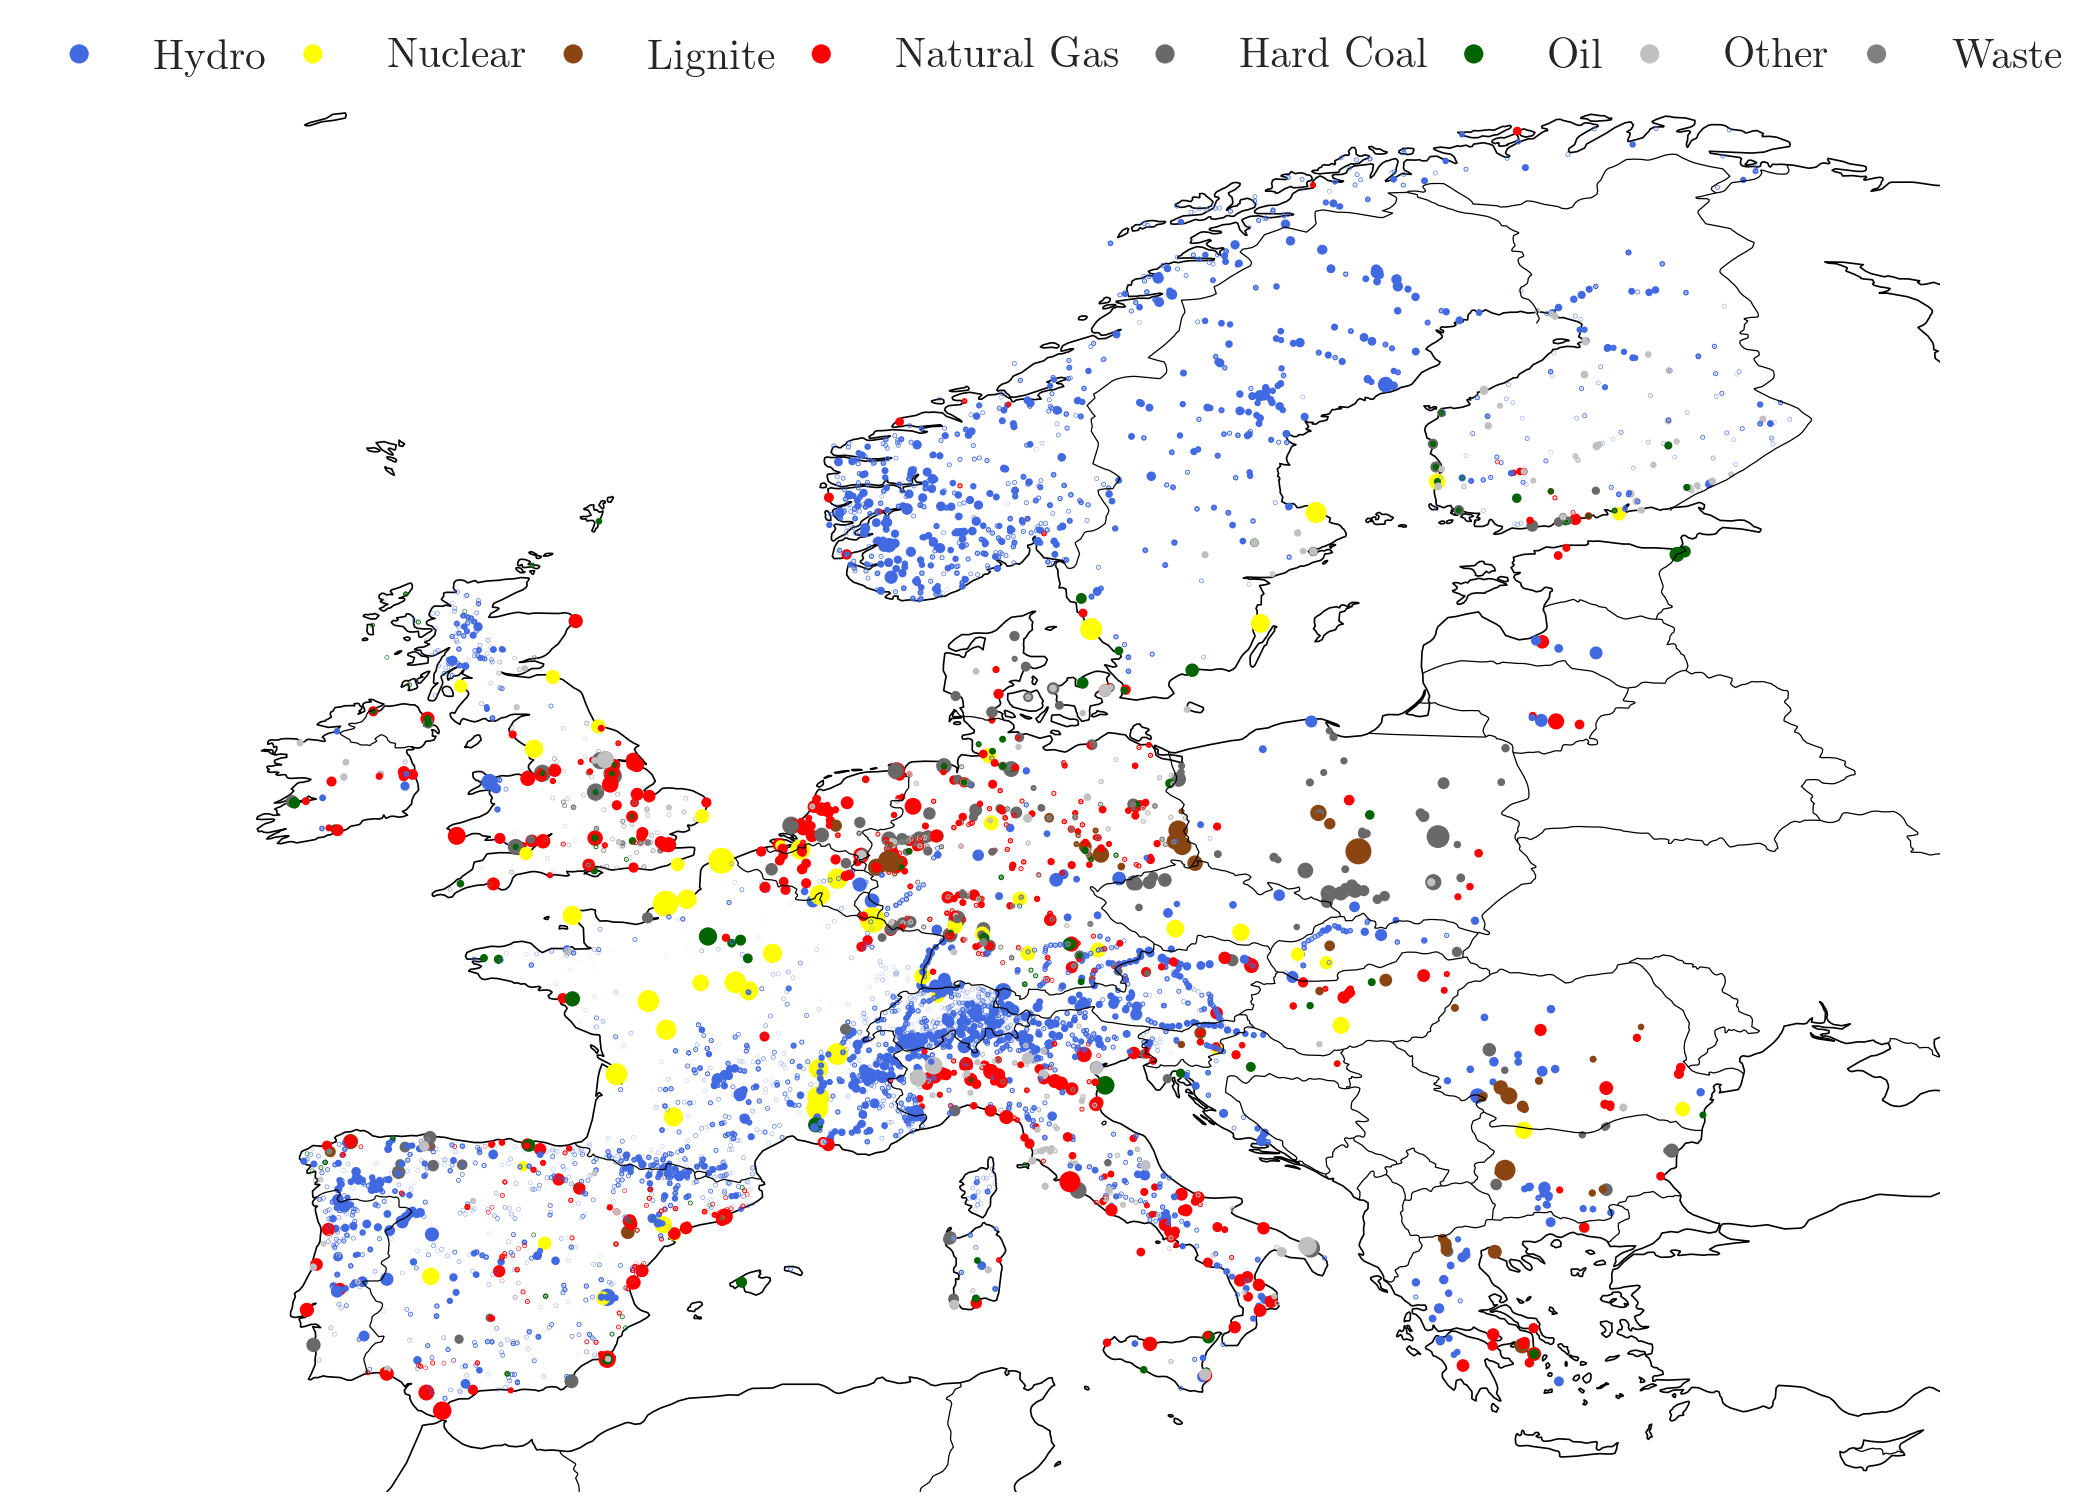
\includegraphics[width=8cm]{images/powerplantmatching.png}

\vspace{0.1cm}
\hrefc{https://github.com/PyPSA/powerplantmatching}{powerplantmatching} tool \\
a showcase example
\end{column}
\end{columns}

\end{frame}

%----------------------------------------
%----------------------------------------

\section{Data sources and key assumptions}

\begin{frame}{Summary of data sources}

  \begin{itemize}
\item Technology data from the open-source \hrefc{https://github.com/PyPSA/technology-data}{technology-data} project \\ (maintained by ENSYS, TU Berlin)
\item Existing generation fleet data from the open-source \hrefc{https://github.com/PyPSA/powerplantmatching}{powerplantmatching} project (maintained by ENSYS, TU Berlin)
\item Renewable power potentials and generation profiles from the open-source \hrefc{https://github.com/PyPSA/atlite}{Atlite} project (maintained by ENSYS, TU Berlin)
\item National climate \& renewable policies:  \\ https://ec.europa.eu for NECPs, https://beyond-coal.eu/, https://world-nuclear.org/
\item Other is based on open-sourced power system data of PyPSA-Eur(-Sec) suite of models \hrefc{https://pypsa.org/}{PyPSA}
  \end{itemize}

\end{frame}


\begin{frame}{Scenario space at one glance}
\centering

\begin{itemize}
    \item Years (2): 2025 and 2030
    \item Zones (4): IE, DK1, DE, NL
    \item Tech palettes (3): \\
        \emph{Palette 1}: wind, solar, battery  storage \\
        \emph{Palette 2}: all above and long-duration energy storage (hydrogen storage system) \\
        \emph{Palette 3}: all above and clean dispatchable generator (advanced geothermal system)
    \item Participation (2): 10\% and 25\% of C\&I load 
    \item Procurement targets (9): (i) different thresholds for
meeting the hourly 24/7 CFE [75\%..100\%], (ii) 100\% annual matching, and (iii) a reference case when 24/7 participants cover load purely with grid purchases
\end{itemize}

\end{frame}


%---------------------------------------------
%---------------------------------------------
\section{Modelling results}


\begin{frame}{Scenario: Participation 25\% - 2025 - IE - Palette 1 
\\ Fraction of demand met with carbon-free energy (CFE)}
\begin{columns}[T]
\begin{column}{9cm}
\centering

\includegraphics[width=9.9cm]{pr/25-2025-IE-p1-used.pdf}
\end{column}
\begin{column}{5cm}

  \begin{itemize}
  \item 100\% RES has only \alert{annual matching}
  \item 100\% RES PPA covers \alert{only 80\%} of hourly demand with CFE
  \item CFE target \alert{90\%} and beyond yields higher share of hourly demand met with CFE
  \item When CFE target approaches 100\%, C\&I participants rely \alert{only on procured resources}
  \end{itemize}
  
\end{column}
\end{columns}

\end{frame}



\begin{frame}{Scenario: Participation 25\% - 2025 - IE - Palette 1
\\ C\&I emission rate}

\begin{columns}[T]
\begin{column}{9cm}
\centering

\includegraphics[width=9.9cm]{pr/25-2025-IE-p1-ci_emisrate.pdf}
\end{column}
\begin{column}{5cm}

  \vspace{.5cm}

  \begin{itemize}
  \item CFE targets beyond \alert{85\%} yield lower emission rate than 100\% RES 
  \item As CFE target is tightened further, average emissions \alert{drop to zero}
  \end{itemize}
\end{column}
\end{columns}

\end{frame}



\begin{frame}{Scenario: Participation 25\% - 2025 - IE - Palette 1 \\
Cost breakdown with existing technologies (wind, solar, battery)}

\begin{columns}[T]
\begin{column}{9cm}
\centering

\includegraphics[width=9.9cm]{pr/25-2025-IE-p1-ci_costandrev.pdf}
\end{column}
\begin{column}{5cm}

  \vspace{.5cm}

  \begin{itemize}
  \item 100\% RES builds wind and solar
  \item Higher CFE targets \alert{include battery storage}
  \item 98\% CFE has \alert{cost premium of only 38\%} over 100\% RES
  \item Last 2\% more than \alert{doubles cost}
  \end{itemize}
\end{column}
\end{columns}

\end{frame}



\begin{frame}{Scenario: Participation 25\% - 2025 - IE - Palette 2 \\
Cost breakdown with long duration energy storage (LDES)}

\begin{columns}[T]
\begin{column}{9cm}
\centering

\includegraphics[width=9.9cm]{pr/25-2025-IE-p2-ci_costandrev.pdf}
\end{column}
\begin{column}{5cm}

  \vspace{.5cm}

  \begin{itemize}
  \item LDES (here 2.5 €/kWh hydrogen storage in caverns), significantly \alert{limits PPA cost increase}
  \item Cost premium of 98\% CFE is reduced to \alert{20\%} above 100\% RES
  \item 100\% CFE is \alert{only 34\%} above 100\% RES
  \end{itemize}
\end{column}
\end{columns}

\end{frame}


\begin{frame}{Scenario: Participation 25\% - 2025 - IE - Palette 3 \\
Cost breakdown with advanced dispatchable generators}

\begin{columns}[T]
\begin{column}{9cm}
\centering

\includegraphics[width=9.9cm]{pr/25-2025-IE-p3-ci_costandrev.pdf}
\end{column}
\begin{column}{5cm}


  \begin{itemize}
  \item Advanced geothermal could \alert{further limit cost}
  \item Firm generation could \alert{remove CFE cost premium}
  \item Results very \alert{sensitive} to cost assumptions (here overnight cost for AGS is at $10.000$~€/kW)
  \item NB Inclusion of clean firm generation reduces storage requirements and limits excess energy
  \item 
  \end{itemize}
\end{column}
\end{columns}

\end{frame}



\begin{frame}{Scenario: Participation 25\% - 2025 - IE - Palette 1 \\
System emissions (full ENTSO-E area),  1/2}

\begin{columns}[T]
\begin{column}{9cm}
\centering

\includegraphics[width=9.9cm]{pr/25-2025-IE-p1-system_emissions.pdf}
\end{column}
\begin{column}{5cm}

  \begin{itemize}
   \item  Here 550~MW of C\&I load in Ireland follows different procurement strategies
   \item 100\% RES can deliver greater system-level CO2 emissions reductions than lower CFE scores
   \item \alert{System emissions reduce} with higher CFE scores, as system-friendly CFE eats into fossil backup in system

  \end{itemize}
\end{column}
\end{columns}

\end{frame}


\begin{frame}{Scenario: Participation 25\% - 2025 - IE - Palette 1 \\
System-level emissions (full ENTSO-E area), 2/2}

\begin{columns}[T]
\begin{column}{9cm}
\centering

\includegraphics[width=9.9cm]{pr/25-2025-IE-p1-system_emissions.pdf}
\end{column}
\begin{column}{5cm}

  \begin{itemize}
   \item  Here 550~MW of C\&I load in Ireland follows different procurement strategies
   \item 100\% RES can deliver greater system-level CO2 emissions reductions than lower CFE scores
   \item \alert{Beyond 85\% CFE score}, 24/7 approach reduce system emissions to a greater extent than 100\% annual matching

  \end{itemize}
\end{column}
\end{columns}

\end{frame}

%----------------------------------------
%now explore IE-2030

\begin{frame}{The impacts of 2030 scenario  \\ 
Fraction of demand met with carbon-free energy (CFE) }

\begin{columns}[T]
\begin{column}{9cm}
\centering

\includegraphics[width=9.9cm]{pr/25-2025-IE-p1-used.pdf}
\end{column}
\begin{column}{5cm}

  \begin{itemize}
  \item Here results showed above for 25\%-\alert{2025}-IE-Palette~1
  \end{itemize}
  
\end{column}
\end{columns}

\end{frame}



\begin{frame}{The impacts of 2030 scenario \\ 
Fraction of demand met with carbon-free energy (CFE) }

\begin{columns}[T]
\begin{column}{9cm}
\centering

\includegraphics[width=9.9cm]{pr/25-2030-IE-p1-used.pdf}
\end{column}
\begin{column}{5cm}

  \begin{itemize}
  \item Here results showed above for 25\%-\alert{2025}-IE-Palette~1
  \item ... 25\%-\alert{2030}-IE-Palette~1
  \item 
  \end{itemize}
  
\end{column}
\end{columns}

\end{frame}


\begin{frame}{The impacts of 2030 scenario  \\ 
Fraction of demand met with carbon-free energy (CFE) }

\begin{columns}[T]
\begin{column}{9cm}
\centering

\includegraphics[width=9.9cm]{pr/25-2030-IE-p2-used.pdf}
\end{column}
\begin{column}{5cm}

  \begin{itemize}
  \item Here results showed above for 25\%-\alert{2025}-IE-Palette~1
  \item ... 25\%-\alert{2030}-IE-Palette~1
  \item ... 25\%-\alert{2030}-IE-Palette~2 (notice how LDES impacts 100\% CFE in 2030, which is not the case in 2025)
  \end{itemize}
  
\end{column}
\end{columns}

\end{frame}


\begin{frame}{The impacts of 2030 scenario  \\ 
Fraction of demand met with carbon-free energy (CFE) }

\begin{columns}[T]
\begin{column}{9cm}
\centering

\includegraphics[width=9.9cm]{pr/25-2030-IE-p3-used.pdf}
\end{column}
\begin{column}{5cm}

  \begin{itemize}
  \item Here results showed above for 25\%-\alert{2025}-IE-Palette~1
  \item ... 25\%-\alert{2030}-IE-Palette~1
  \item ... 25\%-\alert{2030}-IE-Palette~2 (notice how LDES impacts 100\% CFE in 2030, which is not the case in 2025)
 \item ... 25\%-\alert{2030}-IE-Palette~3 (with clean firm generation)
  \end{itemize}
  
\end{column}
\end{columns}

\end{frame}


\begin{frame}{The impacts of 2030 scenario\\
Intuitive effect on all metrics (selected: cost breakdown for Palette 2)}

\begin{columns}[T]
\begin{column}{9cm}
\centering

\includegraphics[width=9.9cm]{pr/25-2030-IE-p2-ci_costandrev.pdf}
\end{column}
\begin{column}{5cm}

  \begin{itemize}
  \item Electricity market developments from 2025 to 2030 (such as technology cost developments, national policies) \alert{decrease PPA cost}
  \item This also \alert{affects cost premium} of CFE vs 100\% annual matching 
  \item In this case, 100\% CFE cost decrease by 12\% compared to 2025 level, while 100\%~RES cost only by 5\%
 
  \end{itemize}
\end{column}
\end{columns}

\end{frame}

%----------------------------------------
%now jump to other countries for selected scenario branches 


\begin{frame}{The impacts of zone where C\&I participants are located}
\centering

Results for scenarios when C\&I load located in other zones show \alert{similar trends.} \\ 
However, each zone is has \alert{unique characteristics} that depend on local resources, national policies, interconnections, etc.

\end{frame}


%----------------------------------------

\begin{frame}{e.g. Germany (25\% - 2025 - DE - Palette~3) 
\\ Fraction of demand met with carbon-free energy (CFE)}

\begin{columns}[T]
\begin{column}{9cm}
\centering

\includegraphics[width=9.9cm]{pr/25-2025-DE-used.pdf}
\end{column}
\begin{column}{5cm}

  \begin{itemize}
  \item German grid is cleaner, in particular due to good interconnections with e.g., France and Denmark
  \item Similar trends to Irish results
  \end{itemize}
  
\end{column}
\end{columns}

\end{frame}

\begin{frame}{e.g. Germany (25\% - 2025 - DE - Palette~3) 
\\ C\&I emission rate}

\begin{columns}[T]
\begin{column}{9cm}
\centering

\includegraphics[width=9.9cm]{pr/25-2025-DE-ci_emisrate.pdf}
\end{column}
\begin{column}{5cm}

  \begin{itemize}
  \item German grid is cleaner, in particular due to good interconnections with e.g., France and Denmark
  \item Similar trends to Irish results
  \end{itemize}
  
\end{column}
\end{columns}

\end{frame}


\begin{frame}{e.g. Germany (25\% - 2025 - DE - Palette~3) 
\\ Cost breakdown with advanced dispatchable generators}

\begin{columns}[T]
\begin{column}{9cm}
\centering

\includegraphics[width=9.9cm]{pr/25-2025-DE-ci_costandrev.pdf}
\end{column}
\begin{column}{5cm}

  \begin{itemize}
  \item German grid is cleaner, in particular due to good interconnections with e.g., France and Denmark
  \item Similar trends to Irish results
  \end{itemize}
  
\end{column}
\end{columns}

\end{frame}


\begin{frame}{e.g. Germany (25\% - 2025 - DE - Palette~3) 
\\ Procured capacity by C\&I participants}

\begin{columns}[T]
\begin{column}{9cm}
\centering

\includegraphics[width=9.9cm]{pr/25-2025-DE-ci_capacity.pdf}
\end{column}
\begin{column}{5cm}

  \begin{itemize}
  \item  One of the unique features of German zone is it's size
  \item Here ca. \alert{9.6~GW} of C\&I load follows different procurement strategies
  \item This leads to relatively \alert{large amount of resources coming into system additionally} due to 24/7 procurement
  \end{itemize}
  
\end{column}
\end{columns}

\end{frame}



\begin{frame}{e.g. Germany (25\% - 2025 - DE - Palette~3) 
\\ Generation of resources procured by C\&I participants}

\begin{columns}[T]
\begin{column}{9cm}
\centering

\includegraphics[width=9.9cm]{pr/25-2025-DE-ci_generation.pdf}
\end{column}
\begin{column}{5cm}

  \begin{itemize}
  \item  One of the unique features of German zone is it's size
  \item Here ca. \alert{9.6~GW} of C\&I load follows different procurement strategies
  \item This leads to relatively \alert{large amount of resources coming into system additionally} due to 24/7 procurement
  \end{itemize}
  
\end{column}
\end{columns}

\end{frame}



\begin{frame}{e.g. Germany (25\% - 2025 - DE - Palette~3) 
\\ System-level capacity difference (rel. to reference scenario)}

\begin{columns}[T]
\begin{column}{9cm}
\centering

\includegraphics[width=9.9cm]{pr/25-2025-DE-total_capacity_diff.pdf}
\end{column}
\begin{column}{5cm}

  \begin{itemize}
  \item  Clean capacity procured by C\&I customers displaces capacity built in the rest of the system 
  \item Here remarkable that \alert{C\&I clean resources substitute gas-fired technology}
  \item Inclusion of clean firm resources in C\&I portfolio \alert{helps to decarbonise} the entire electricity system
  \end{itemize}
  
\end{column}
\end{columns}

\end{frame}


%---------------------------------------------
%---------------------------------------------
\section{Additional scenarios}


\begin{frame}{The special scenario case}
\centering

Results for Denmark are pretty special. \\
This is driven by the Danish \hrefc{https://energy.ec.europa.eu/system/files/2020-01/dk_final_necp_main_en_0.pdf}{national energy and climate policy} \\ 
aimed at 110\% of renewable electricity in the consumption mix by 2030.

\end{frame}


\begin{frame}{Scenario: 25\% - 2030 - DK1 - Palette~2
\\ Fraction of demand met with carbon-free energy (CFE)}

\begin{columns}[T]
\begin{column}{9cm}
\centering

\includegraphics[width=9.9cm]{pr/25-2030-DK-p2-used.pdf}
\end{column}
\begin{column}{5cm}

\begin{itemize}
  \item Danish grid in 2030 is \alert{extremely clean}
  \item Only \alert{CFE scores above 95\%} deliver higher fraction of demand met with carbon-free energy than 100\% annual matching
\end{itemize}
  
\end{column}
\end{columns}

\end{frame}


\begin{frame}{Scenario: 25\% - 2030 - DK1 - Palette~2 \\ 
C\&I emission rate}

\begin{columns}[T]
\begin{column}{9cm}
\centering

\includegraphics[width=9.9cm]{pr/25-2030-DK-p2-ci_emisrate.pdf}
\end{column}
\begin{column}{5cm}

\begin{itemize}
  \item Danish grid in 2030 is \alert{extremely clean}
  \item Similar picture can be seen with the average emissions -- only \alert{CFE scores above 95\%} yield lower emission rate
  \item Even the reference case is at incredible 30~kg/MWh emission rate
\end{itemize}
  
\end{column}
\end{columns}

\end{frame}


\begin{frame}{Scenario: 25\% - 2030 - DK1 - Palette~2 \\ 
Cost breakdown with advanced dispatchable generators}

\begin{columns}[T]
\begin{column}{9cm}
\centering

\includegraphics[width=9.9cm]{pr/25-2030-DK-p2-ci_costandrev.pdf}
\end{column}
\begin{column}{5cm}

\begin{itemize}
  \item Danish grid in 2030 is \alert{extremely clean}
  \item The PPA cost is below 80~€/MWh level with just the LDES technology
\end{itemize}
  
\end{column}
\end{columns}

\end{frame}


%----------------------------------------
\section{Discussion \& Takeaways}


\begin{frame}{Discussion:}

  \begin{itemize}
  \item 24/7 CFE procurement in Europe \alert{reduces emissions} both for buyer and for rest of system. The level of emission reduction is subject to zone where C\&I participants are located, as well as the time period.
  \item 75-90\% hourly CFE targets have \alert{only small cost premium} over annual RES matching.
  \item 100\% hourly CFE target \alert{comes at costs}. However, LDES can considerably decrease the cost premium. Inexpensive clean firm generation could nearly remove the cost premium.   
  \item 24/7 approach \alert{triggers investment in new technologies} the system will need later: long-duration storage and dispatchable clean generation.
  \item 24/7 approach \alert{benefits the rest of the system}, reducing emissions and flexibility needs.
  \end{itemize}

\end{frame}

%----------------------------------------
%----------------------------------------
\section*{Backup}

\begin{frame}{Code availability}

  The code is already available online with an MIT licence:

  \urlc{https://github.com/PyPSA/247-cfe}

\end{frame}


\begin{frame}
  \frametitle{24/7 carbon-free procurement}

  Idea behind \alert{24/7 carbon-free energy (CFE)} procurement:

  \begin{itemize}
  \item Insist that contracted power is \alert{additional} (i.e. leads to new capacity)
  \item Insist power comes from the \alert{same bidding zone}
   \item Insist that demand is matched on an \alert{hourly basis}
    \item Insist that power is \alert{carbon-free} rather than renewable (i.e. technology neutrality)
  \end{itemize}

\end{frame}


\begin{frame}{Implementation of C\&I demand and supply}

  The hourly C\&I demand $d_t$ for hour $t$ can be met by procured CFE generators $r\in CFE$ dispatching $g_{r,t}$~MW but also storage discharging $\bar{g}_{s,t}$ and charging $\ubar{g}_{s,t}$ for storage technologies $s\in STO$ as well as from imports from the grid $im_t$. The excess from the local supply $ex_t$ can either be sold to the grid or curtailed
  \begin{equation*}
  \sum_{r\in CFE} g_{r,t} + \sum_{s\in STO} \left(\bar{g}_{s,t} - \ubar{g}_{s,t}\right) - ex_t + im_t  =  d_t \hspace{.7cm} \forall t
  \end{equation*}

\centering
\begin{circuitikz}
  \draw (0,13.5) to [short,i^=$im_t$]  (1.5,13.5) to (1.5,13);
  \draw [ultra thick] (0,13) node[anchor=south]{} -- (4,13);
  \draw(2.5,13) |- +(0,0.5) to [short,i^=$ex_t$] +(1.5,0.5);
  \draw (0.5,13) -- +(0,-0.5) node[sground]{};
  \draw (2,12) node[vsourcesinshape, rotate=270](V2){}
  (V2.left) -- +(0,0.6);
  \draw (3.5,13) -- (3.5,12.4);
  \draw (3.5,12.4) to [esource] (3.5,11.7);
  \draw (0.5,11) node{$d_t$};
  \draw (2,11) node{$g_{CFE,t}$};
  \draw (3.5,11) node{$g_{STO,t}$};
\end{circuitikz}

\end{frame}


\begin{frame}{Methodology for RES and CFE constraints, 1/2}

  The 100\% \alert{RES constraint} ensures that the sum of all dispatch $g_{r,t}$ for RES generators $r\in RES$ over the year $t\in T$ is equal to the sum of demand $d_t$ at the data center
  \begin{equation*}
    \sum_{r\in RES, t\in T} g_{r,t} = \sum_{t\in T} d_t
  \end{equation*}

\end{frame}


\begin{frame}{Methodology for RES and CFE constraints, 2/2}


  The $x \cdot 100$\% \alert{carbon-free energy (CFE) constraint} sums over CFE generators $r\in CFE$ but also storage discharging $\bar{g}_{s,t}$ and charging $\ubar{g}_{s,t}$ for storage technologies $s\in STO$ as well as the excess from the data center $ex_t$ (could be sold to grid or curtailed) and import from the grid $im_t$ multiplied by the grid's CFE factor $CFE_t$ (the fraction of CFE technology running at time $t$)
  \begin{equation*}
  \sum_{r\in CFE, t\in T} g_{r,t} + \sum_{s\in STO, t\in T} \left(\bar{g}_{s,t} - \ubar{g}_{s,t}\right) - \sum_{t\in T} ex_t + \sum_{t\in T} CFE_t \cdot im_t \geq x \cdot \sum_{t\in T} d_t
  \end{equation*}

  \begin{equation*}
  \sum_{t\in T} ex_t \leq ExLimit \cdot \sum_{t\in T} d_t
  \end{equation*}

\begin{itemize}
    \item  The grid CFE factor $CFE_t$ is affected by capacity built at data center, so has to be updated iteratively (starting with $CFE_t =0 \, \forall t$, convergence is very good after 1 iteration).
    \item Annual excess generation is constrained to 80 percentage points less than the annual CFE target per year, i.e. $ExLimit = max(0, x - 0.8)$. This sets 10\% limit for 90\% CFE, 
     and 20\% for 100\% CFE.
\end{itemize}



\end{frame}


\begin{frame}
  \frametitle{Python for Power System Analysis: Worldwide Usage}

  PyPSA is used worldwide by \alert{dozens of research institutes and companies} (TU Delft, KIT, Shell, TSO TransnetBW, TERI, Agora Energiewende, RMI, Fraunhofer ISE, Climate Analytics, DLR, FZJ, RLI, Saudi Aramco, Edison Energy, spire and many others). See \hrefc{https://pypsa.readthedocs.io/en/latest/users.html}{list of users}.

  \centering
  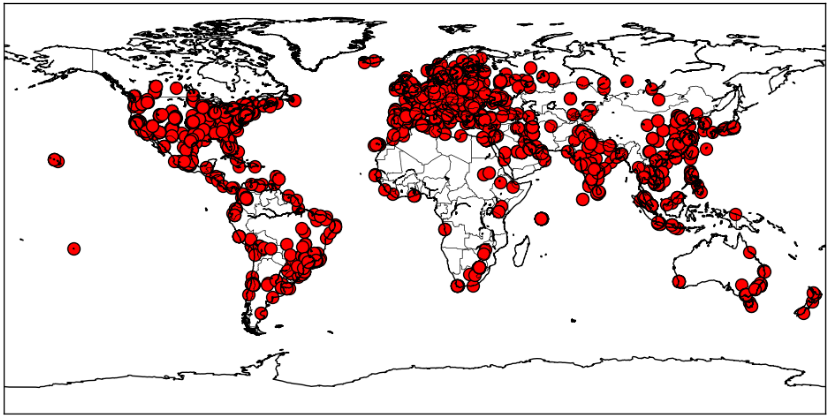
\includegraphics[width=12cm]{images/users.png}

\end{frame}


\begin{frame}
  \frametitle{PyPSA-Eur: Open Model of European Energy System}
\begin{columns}[T]
\begin{column}{6cm}

  \vspace{0.3cm}
\centering

%\includegraphics[width=4cm]{line-loading}
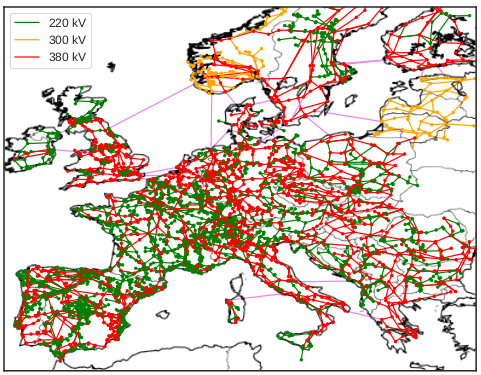
\includegraphics[width=7cm]{images/pypsa-eur-grid.png}

\vspace{.1cm}

Basic \alert{validation} of grid model in \hrefc{https://arxiv.org/abs/1806.01613}{Hörsch et al, 2018)},
\hrefc{https://github.com/PyPSA/pypsa-eur}{github.com/PyPSA/pypsa-eur}

\end{column}
\begin{column}{7.5cm}

  \begin{itemize}
    \item Grid data based on \alert{GridKit} extraction of ENTSO-E interactive map
    \item \alert{powerplantmatching} tool combines open databases using matching algorithm \href{https://github.com/larsga/Duke}{DUKE}
    \item Renewable energy time series from open \alert{atlite}, which processes terabytes of weather data from e.g. new ERA5 global reanalysis
    \item Geographic \alert{potentials} for RE from land use GIS availability
    \item All energy demand and supply options (power, transport, heating and industry)
      \item  See \hrefc{https://docs.google.com/presentation/d/1mzj4X9uuO58gUvkhVMRCFWOJUWbs6NR9SNZe-RIkkNo/edit?usp=sharing}{other slidedeck} for full details

  \end{itemize}
\end{column}
\end{columns}

\end{frame}



\begin{frame}
  \frametitle{More information}

  All input data and code for PyPSA-Eur-Sec is open and free to download:
  \begin{enumerate}
  \item \url{https://github.com/pypsa/pypsa}: The modelling framework
  \item \url{https://github.com/pypsa/pypsa-eur}: The power system model for Europe
  \item \url{https://github.com/pypsa/pypsa-eur-sec}: The full energy system model for Europe
  \end{enumerate}

  \vspace{.3cm}

  Publications (selection):
  {\tiny
    \begin{enumerate}
      \item M.~Victoria, K.~Zhu, T.~Brown, G.~B.~Andresen, M.~Greiner, \emph{``Early decarbonisation of the European energy system pays off,''} Nature Communications (2020),  \hrefc{https://doi.org/10.1038/s41467-020-20015-4}{DOI}, \hrefc{https://arxiv.org/abs/2004.11009}{arXiv}.
  \item T.~Brown, D.~Schlachtberger, A.~Kies, S.~Schramm, M.~Greiner, \emph{``Synergies of sector coupling and transmission reinforcement in a cost-optimised, highly renewable European energy system,''} Energy 160 (2018) 720-739, \hrefc{https://doi.org/10.1016/j.energy.2018.06.222}{DOI}, \hrefc{https://arxiv.org/abs/1801.05290}{arXiv}.
  \item J.~Hörsch, F.~Hofmann, D.~Schlachtberger and T.~Brown, \emph{``PyPSA-Eur: An open optimization model of the
    European transmission system,''} Energy Strategy Reviews (2018), \hrefc{https://doi.org/10.1016/j.esr.2018.08.012}{DOI}, \hrefc{https://arxiv.org/abs/1806.01613}{arXiv}
  \item D.~Schlachtberger, T.~Brown, M.~Schäfer, S.~Schramm, M.~Greiner, \emph{``Cost optimal scenarios of a future highly renewable European electricity system: Exploring the influence of weather data, cost parameters and policy constraints,''} Energy (2018), \hrefc{https://doi.org/10.1016/j.energy.2018.08.070}{DOI}, \hrefc{https://arxiv.org/abs/1803.09711}{arXiv}.
\item T.~Brown, J.~Hörsch, D.~Schlachtberger, \emph{``PyPSA: Python for Power System Analysis,''}  Journal of Open Research Software, 6(1), 2018, \hrefc{https://doi.org/10.5334/jors.188}{DOI}, \hrefc{https://arxiv.org/abs/1707.09913}{arXiv}.
\item D.~Schlachtberger, T.~Brown, S.~Schramm, M.~Greiner, \emph{``The Benefits of Cooperation in a Highly Renewable European Electricity System,''} Energy 134 (2017) 469-481, \hrefc{https://doi.org/10.1016/j.energy.2017.06.004}{DOI}, \hrefc{https://arxiv.org/abs/1704.05492}{arXiv}.
  \end{enumerate}
}
\end{frame}

\end{document}
